\begin{frame}

\begin{center}
Why do we \textbf{search for...}?
\end{center}

\begin{minipage}[c]{.45\textwidth}
\begin{block}{Current standard model status}
\begin{itemize}
\item Robust and predictive (top quark, \Wboson, \Zboson\ and one Higgs boson...)
\item Still not good enough, unable to explain some observations such as:
\begin{itemize}
\item dark matter \only<2>{$\longrightarrow$}
\item matter vs antimatter asymmetry
\item naturalness problem
\item ...
\end{itemize}
\item Go beyond with a new model!
\item Consequences of this new model? \textbf{\color{ltcolorred}Test it!}
\end{itemize}
\end{block}
\end{minipage}
\hfill
\begin{minipage}[c]{.45\textwidth}
\only<2>{\begin{center}
\vspace{\baselineskip}

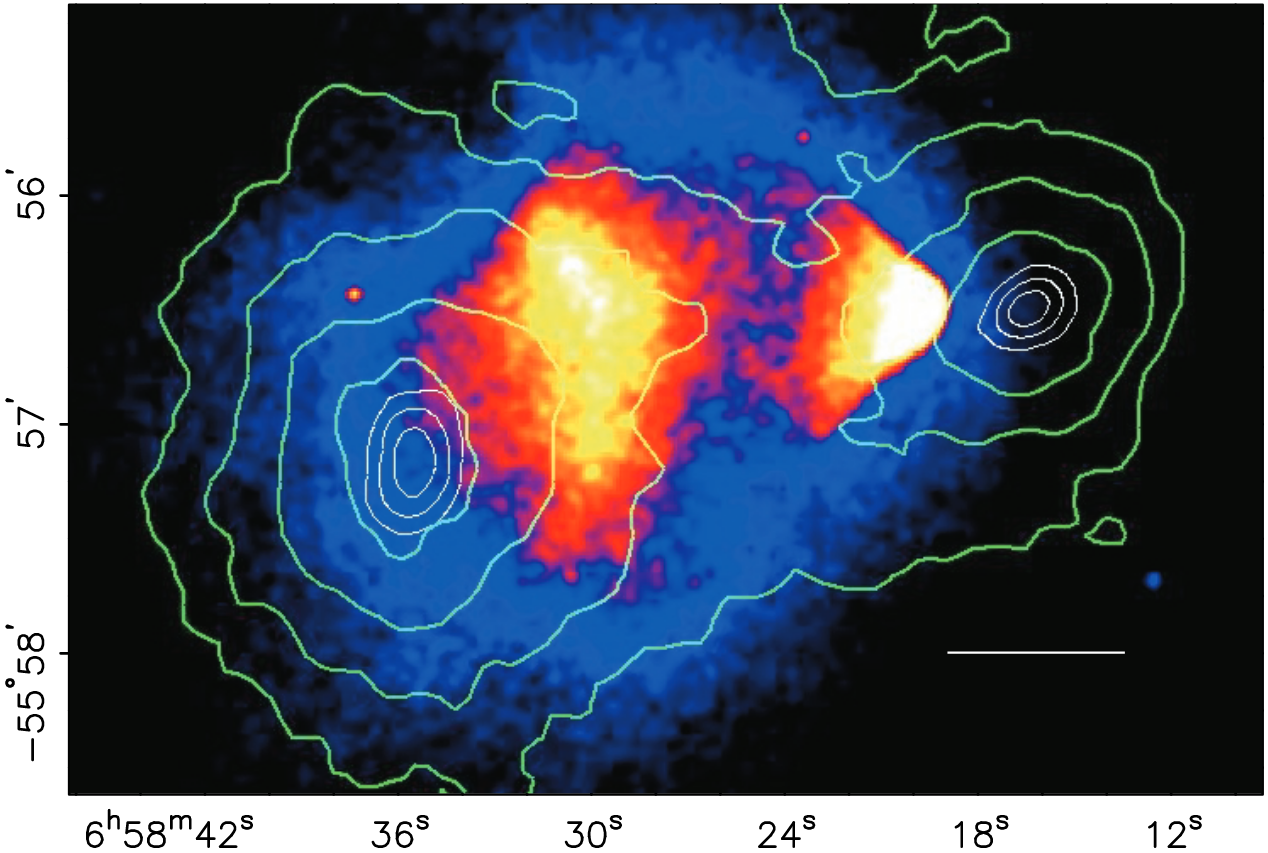
\includegraphics[width=.9\linewidth]{\PhDthesisdir/plots_and_images/from_Clowe_2006/bullet_cluster.png}

Difference due to \textbf{dark matter}!
\end{center}}
\end{minipage}
\beamercite{Clowe_2006}

\begin{tikzpicture}[overlay]
\only<2>{
\draw (.525\textwidth, .65\textheight) node (a) [above right] {Galaxies from:\vphantom{Àq}};
\draw [ltcolorred] (a.east) node [right] (b) {X~rays\vphantom{Àq}};
\draw [ltcolorgreen] (b.east) node [right] (c) {gravitational lensing\vphantom{Àq}};

\draw (.75\textwidth, .45\textheight) coordinate (b1);
\draw (.85\textwidth, .43\textheight) coordinate (b2);
\draw (.7\textwidth, .325\textheight) coordinate (c1);
\draw (.9\textwidth, .44\textheight) coordinate (c2);

\draw [ltcolorred3, thick, -latex] (b) -- (b1);
\draw [ltcolorred3, thick, -latex] (b) -- (b2);
\draw [ltcolorgreen3, thick, -latex] (c) -- (c1);
\draw [ltcolorgreen3, thick, -latex] (c) -- (c2);
}
\end{tikzpicture}
\end{frame}

\begin{frame}{Keywords in title}
\begin{center}
\small
\begin{tikzpicture}
\draw (0,0) node [below right] (t1) {Search for\vphantom{Àq}};
\draw (t1.east) node (t2) [right] {\color{ltcolorblue}\textbf{additional heavy Higgs bosons decaying to tau lepton pair}\vphantom{Àq}};
\draw (t2.east) node (t6) [right] {in the\vphantom{Àq}};
\draw (t6.east) node (t7) [right] {\color{ltcolorred}\textbf{CMS experiment at LHC}\vphantom{Àq}};

\only<2->{
\draw [thick, ltcolorblue] (t2.south east) -- (t2.south west) ;
\draw [thick, ltcolorblue, -latex] (t2.south) --+ (0,-1.5) node (l3) [below] {Part~I\vphantom{Àq}};
\draw  (l3.south) node (l3bis) {\emph{Phenomenology}};
}

\draw (t7.south east) coordinate (0) ;
\only<3->{
\draw [thick, ltcolorred] (t7.south east) -- (t7.south west) ;
\draw [thick, ltcolorred, -latex] (t7.south) --+ (0,-1.5) node (l10) [below] {Part~II\vphantom{Àq}};
\draw  (l10.south) node (l10bis) {\emph{Experimental device}};
}

\only<4->{
\draw ($(l3)!0.5!(l10)$) coordinate (middle);
\draw (middle) + (0, -1.5) node (l12) {Part~III\vphantom{Àq}};
\draw (l12.south) node (l12bis) {\emph{\HAtoTauTau\ analysis}};
\draw [thick, -latex] (l3bis) -- (l12.west) ;
\draw [thick, -latex] (l10bis) -- (l12.east) ;
}

\only<5->{
\draw (l12bis) + (0, -1.5) node {+ Part~IV: \color{ltcolorviolet}\textbf{with machine learning techniques}};
}

\draw (.5\textwidth,-.75\textheight) coordinate (a);
\end{tikzpicture}
\end{center}
\end{frame}